\documentclass[11pt]{article}
\newcommand{\numpy}{{\tt numpy}}    % tt font for numpy
\usepackage[margin=1in]{geometry}
\usepackage{hyperref}
\usepackage{graphicx}
\hypersetup{
    colorlinks=true,
    linkcolor=cyan,
    filecolor=magenta,      
    urlcolor=blue,
}

\begin{document}

$$\mbox{\Large \textbf {CS 111 (S19): Homework 5}}$$
$$\mbox{\textbf {Due by 6:00 PM, Wednesday, May 15}}$$
$$\mbox{\textbf {NAME and PERM ID No.:} Chen Li, 5468137 }$$
$$\mbox{\textbf {UCSB EMAIL:} chenli@ucsb.edu }$$

\par\bigskip
{\bf 1.}
The moral of this problem is twofold: 
First, linear least squares can be used to fit data with polynomials,
not just with straight lines or planes.
(As we've seen, it can be used to fit data with lots of different kinds of models.)
Second, fitting data with a very high-degree polynomial can be a bad idea.

The data for this problem is the population of the United States at each
10-year census from 1900 to 2010. Here is the data.
\begin{verbatim}
    date = np.array(range(1900,2020,10)) - 1900
    population = 1000 * np.array([ 75995,  91972, 105711, 123203, 131669, 150697, 
                                  179323, 203212, 226505, 249633, 281422, 308746])
    for (d,p) in zip(date, population):
        print(d, ':', p)
\end{verbatim}
(Notice that we are writing the date as ``years since 1900.''
How come?
It turns out to make the fitting computation more stable.
We may return to this in the next homework.)

\par\medskip
{\bf 1a.}
Express the problem of fitting a straight line of the form
$$ p = x_0 + x_1d$$
to the data as a linear least squares problem
$$A x \approx b$$
where $x = (x_0, x_1)^T$ is the vector of coefficients of the line.
(The answer to this question consists just of the 12-by-2 matrix $A$ 
and the vector $b$.)$$
A = np.ones((12,2))$$$$
A[:,1]=date
$$$$b = population$$\\
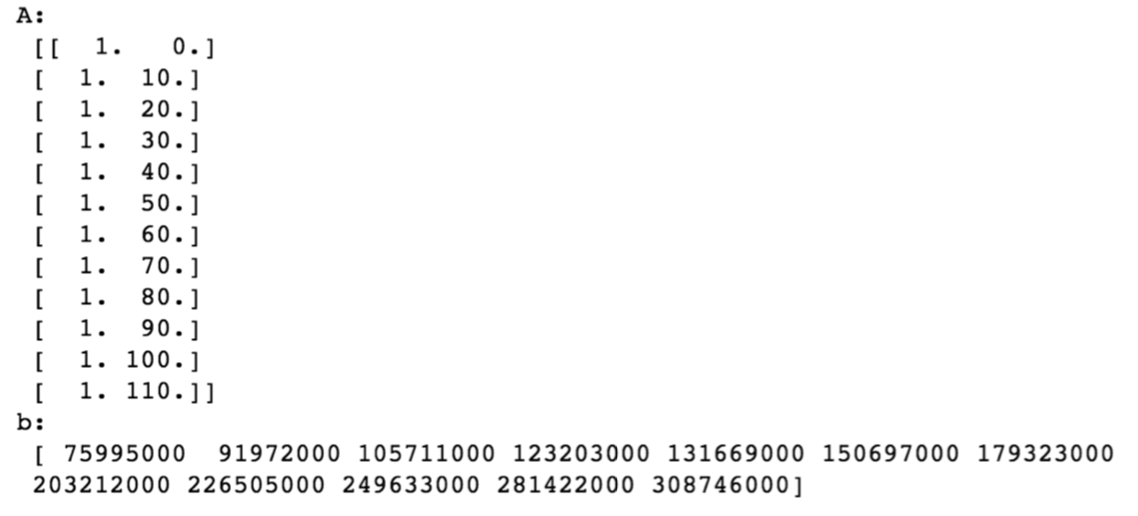
\includegraphics[scale = 0.4]{h51a2}
\par\medskip
{\bf 1b.}
Solve the least squares problem in (5a) for $x$ in two different ways:
First, use the QR factorization of $A$.
Second, use the {\tt scipy} routine {\tt npla.lstsq()}.
(This uses either QR or SVD under the hood, but it has more
bells and whistles; see the python help for the function.
You'll need to give it an extra argument {\tt rcond=None},
and the solution it returns is a python tuple whose first element is $x$.)
Verify that the two $x$ vectors are (nearly) the same.
Make a plot that shows the original population data as circles,
and the least squares fit as a line.\\
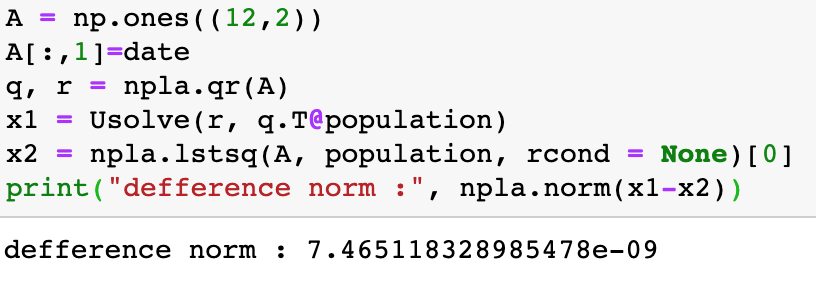
\includegraphics[scale = 0.7]{h51b.png}\\
x=[61330474.35897431, 2109276.22377622]\\
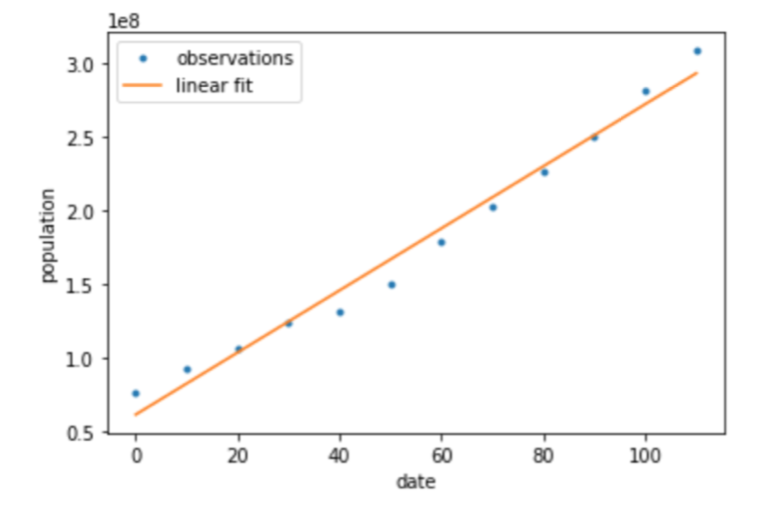
\includegraphics{h51c2.png}date after 1900
\par\medskip
{\bf 1c.}
Use $x$ to compute the US population in the year 2020, 
as predicted by the straight-line fit.\\
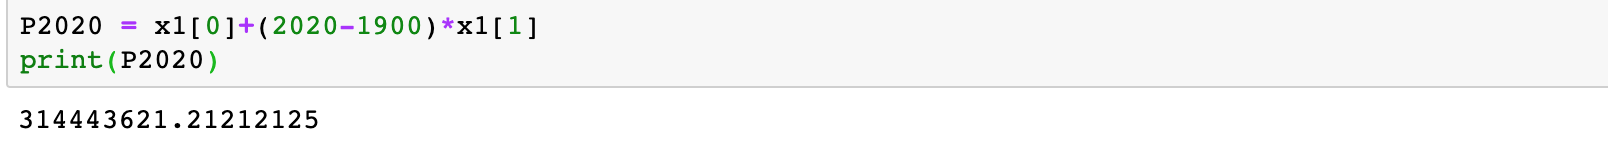
\includegraphics[scale = 0.4]{h51c}

\par\medskip
{\bf 1d.}
Express the problem of fitting a quadratic polynomial of the form
$$ p = x_0 + x_1d + x_2d^2 $$
to the data as a linear least squares problem
$$A x \approx b$$
where $x = (x_0, x_1, x_2)^T$ is the vector of coefficients of the polynomial.
This time the matrix $A$ will be 12-by-3.
Again, solve the least squares problem 
(using your choice of QR factorization or {\tt npla.lstsq()} but not both),
make a plot of the resulting parabola, 
and use the new $x$ to predict the 2020 population.\\
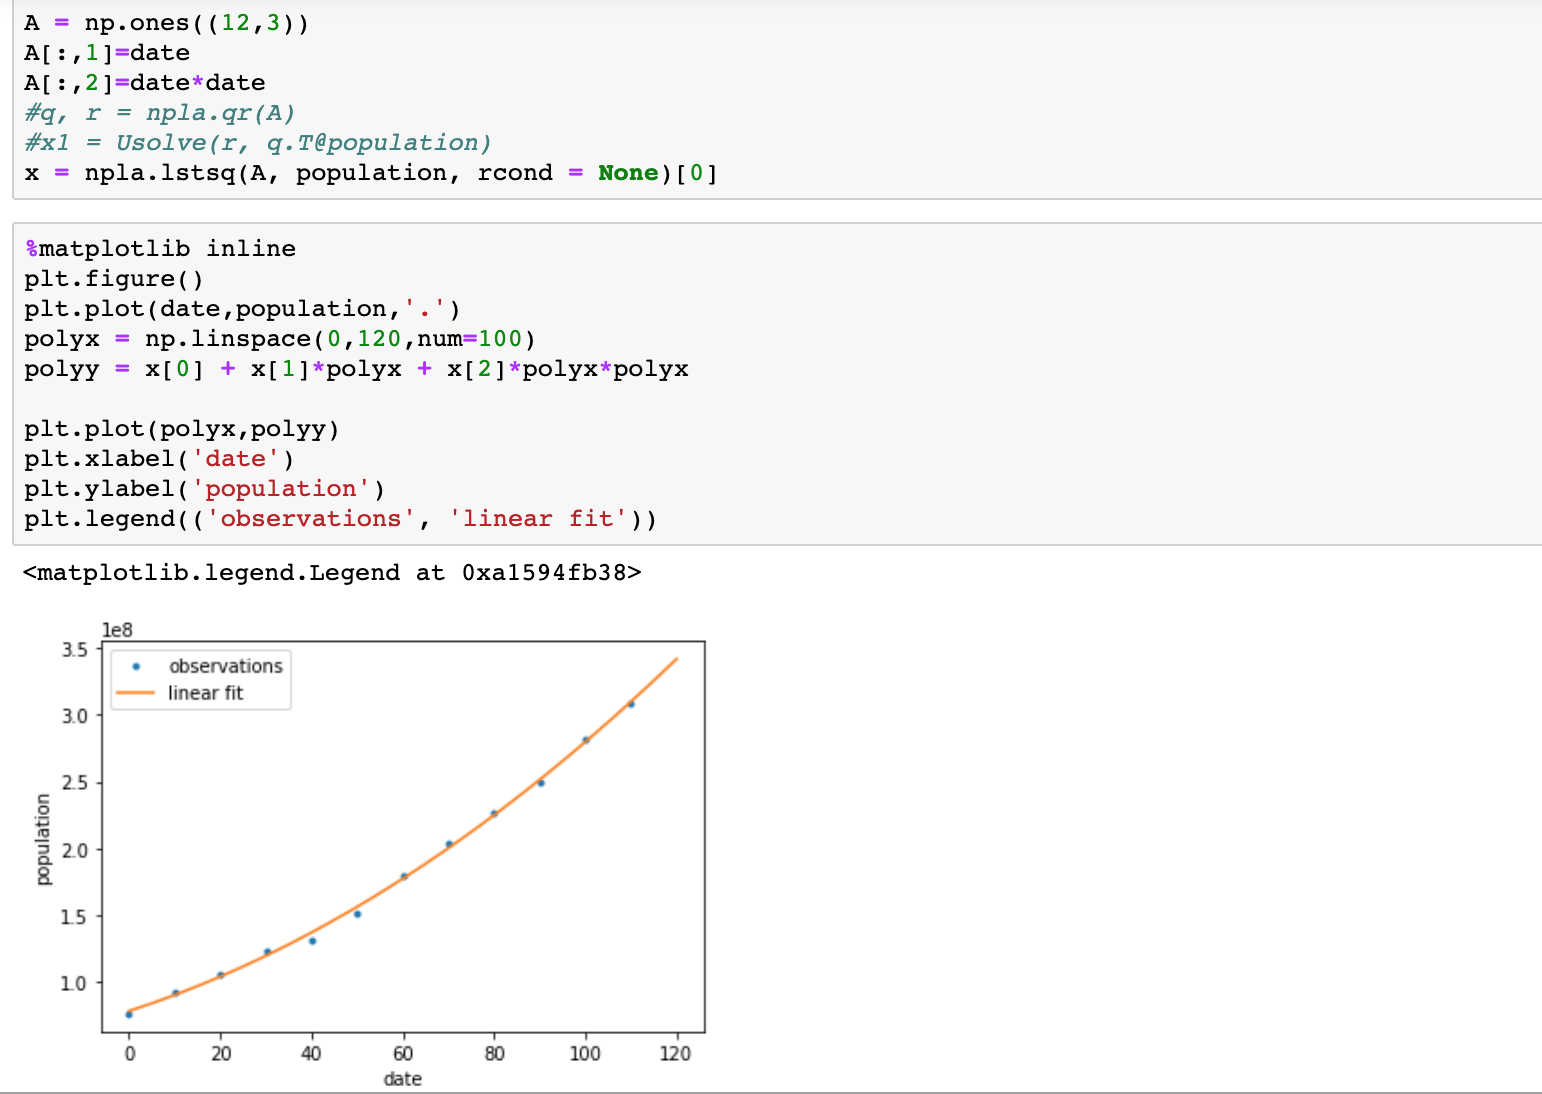
\includegraphics[scale = 0.6]{h51d}\\
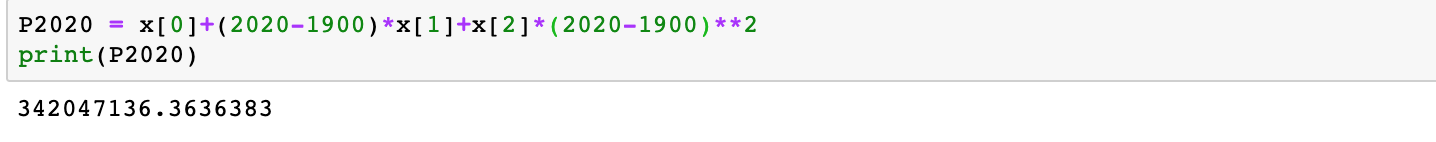
\includegraphics[scale = 0.6]{h51d2.png}\\
x=[7.80139176e+07   1.10826963e+06   9.10005994e+03]
\par\medskip
{\bf 1e.}
Revise the code you used in (1d) to take the polynomial degree as a parameter.
Repeat the fitting, plotting, and prediction 
for polynomials of degrees 3, 4, \ldots, 8.
(Turn in your plots and the values of your predictions for this part,
but not your python code.)
What do you notice about the last few predictions?\\
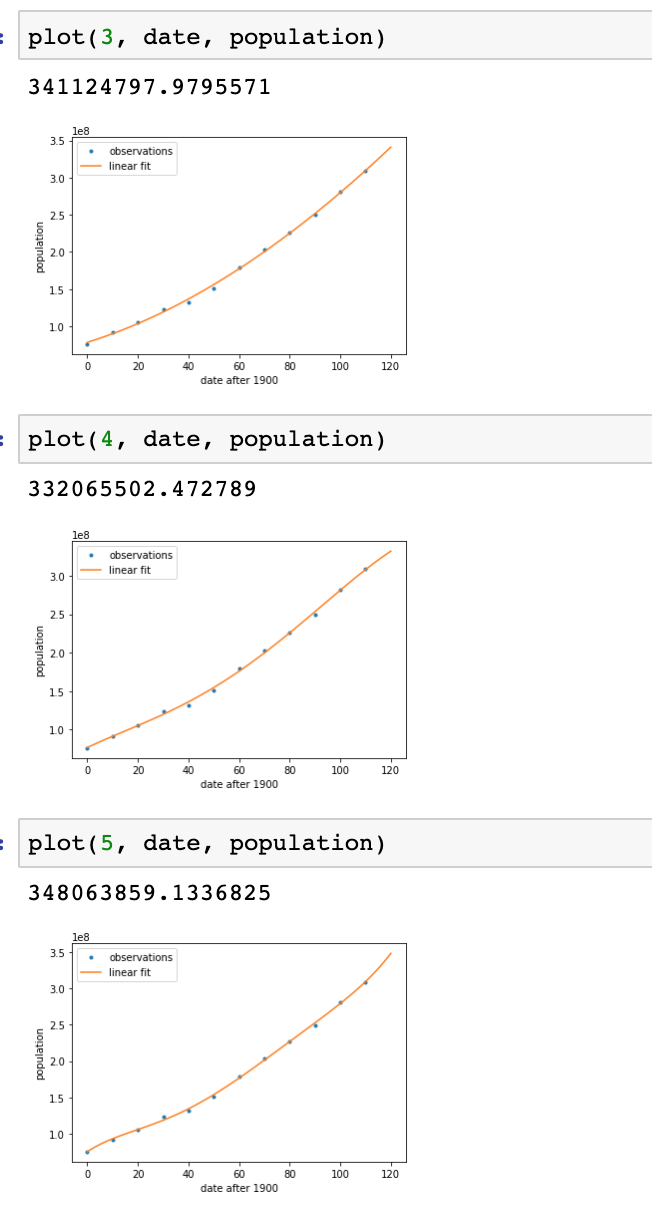
\includegraphics[scale = 0.7]{h51e1.png}
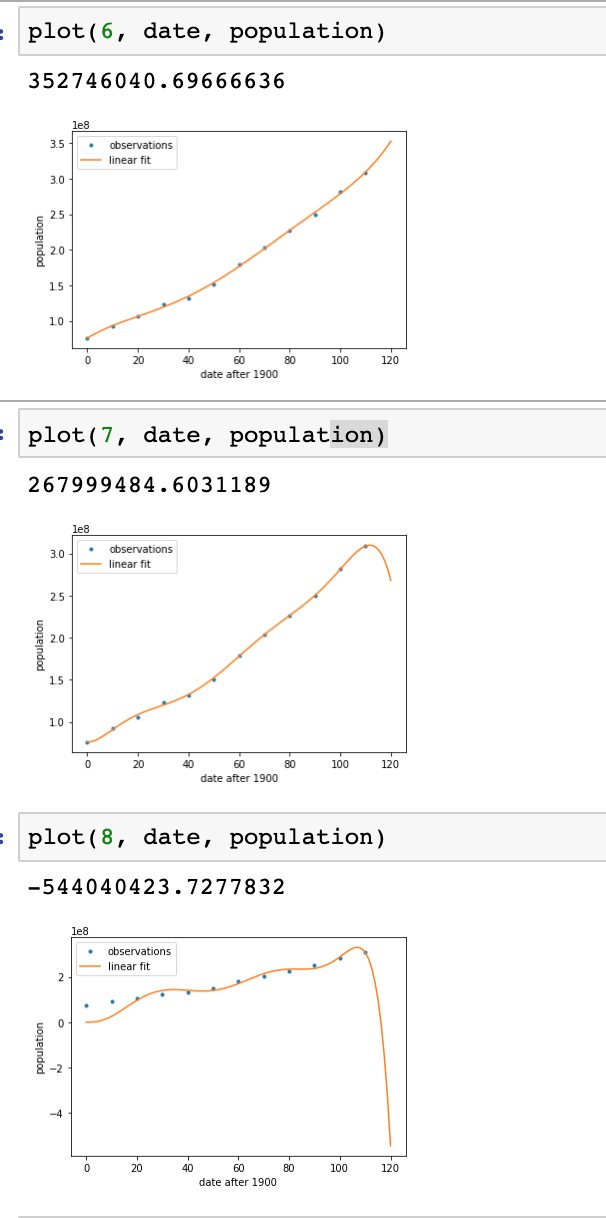
\includegraphics[scale = 0.7]{h51e2}\\
The predicting value are above plot.\\ in the last few predictions, the expected value drops drastically and become ridiculous negative number. The line become more fluctuate and less close.
\par\bigskip
\newpage
{\bf 2.}
These questions are all about IEEE standard 64-bit floating-point arithmetic,
which is behind both numpy's {\tt float64} type and C's {\tt double} type.
You can use {\tt fprint()} from the Feb 4 class to see
the actual bits that represent any number.
Recall that one hexadecimal digit stands for 4 bits.

\par\medskip
{\bf 2a.}
{\em Machine epsilon}, or just $\epsilon$ for short, is defined as the largest
floating-point number $x$ such that $x + 1 = 1$ in floating-point arithmetic.
The experiment we did in class showed that $\epsilon$ is approximately $10^{-16}$,
which is why we say that IEEE floating-point can be accurate to
about 16 decimal digits.

What is the exact value of $\epsilon$? (Your answer should be an exact arithmetic
expression, not a decimal expansion.) What is the 16-digit hex representation of
$\epsilon$ in the IEEE standard? How close is $\epsilon$ to $10^{-16}$?
$$\epsilon = 2^{-53}\approx1.1102230246251565^{-16}=0x3ca0000000000000$$
$$residual = \epsilon-10^{-16}=1.1022302462515656e-17$$
\par\medskip
{\bf 2b.}
What is the 16-digit hex representation of $1/\epsilon$? What is its approximate
value in base 10?\\
$$1/\epsilon  = 0x4340000000000000 \approx 9007199254740992.0$$
\par\medskip
{\bf 2c.}
What is the largest non-infinite positive number that can be represented exactly
in IEEE floating-point? Give your answer three ways: As an exact arithmetic
expression, as the 16-hex-digit IEEE representation, and as an approximate
value in base 10. (Hint: Consider the largest possible value of the 11-bit
exponent field in the IEEE standard, but remember that value is reserved
to represent ``infinity''.)\\\\
In binary, the sign should be 0, the exponent should be 11111111110, mantissa should be all 1s, which is $2^{-52}$ smaller than $2^1$. therefore, the largest should be:$$
(-1)^02^{2046-1023}(2-2^{-52})=0x7fefffffffffffff\approx 1.7976931348623157e+308
$$
\par\medskip
{\bf 2d.}
A common mistake some people make (but not you!) is to think that $\epsilon$ is
the smallest positive floating-point number. It's not, by a long shot. Consider
for example $x = \epsilon^{10}$. What is the approximate value of $x$ in base 10?
Is $x$ an exact floating-point number? If so, give its IEEE 16-hex-digit representation;
if not, give an IEEE 16-hex-digit representation of a floating-point number as
close to $x$ as you can.\\
$$2.8451311993408992e-160$$\\it is an exact floating point
$$0x1ed0000000000000$$

\par\medskip 
{\bf 2e.}
How many different floating-point numbers $x$ are there with $1 < x < 2$?
How many with $4096 < x < 8192$?  How many with $1/64 < x < 1/32$?\\\\
the bounds of each group are different in exponent by one and has the same mantissa, which are all 0s, so there are actually 52 bits to accommodate numbers before its exponent get incremented by 1, so the answers is
$$2^{52}-1, 2^{52}-1,2^{52}-1$$

\par\medskip
{\bf 2f.}
Standard 64-bit integer arithmetic (such as {\tt int64\_t} in C) uses
twos complement to represent integers from roughly $-2^{63}$ to $2^{63}$.
In this system, the number of negative integers is different from the number of
positive integers. Why? Is the number of negative IEEE floating-point numbers
different from the number of positive IEEE floating-point numbers? 
Why or why not?\\\\
For the first question, in standard 64-bit integer arithmetic, 100000000... represent the most negative integer, whereas 00000000... represent 0 rather than most positive integer, so the negative domain can accommodate one more position than positive domain do.\\
For the second question, IEEE floating-point provide same number of positive and negative float points, because there are positive zero and negative zero in this system. Therefore, the only difference is sign and it has same number of positive numbers and negative numbers%baby i love u 
\newpage

\par\bigskip
{\bf 3.}
For this problem, you may want to read the article 
``Tearing apart Google's TPU 3.0 AI coprocessor'' 
(linked from the Feb 4 class notes),
especially the section ``TPU Chips'' that starts on page 8.

The 1985 IEEE floating-point standard specifies a 16-bit version 
and a 32-bit version as well as the ubiquitous 64-bit version.
The 16-bit version was never used much, 
because most scientific modeling requires higher precision. 
Recently, though, 
16-bit floating-point has become popular in machine learning applications,
because the weights in a neural network don't need to be determined very precisely.

IEEE standard 16-bit floating-point uses 1 bit for the sign, 5 bits for 
the exponent, and 10 bits for the mantissa. 
However, when Google developed its TPU (``Tensor Processing Unit'') chip
for machine learning, it used a different 16-bit format that it calls
``bfloat'', with 1 bit for the sign, 8 bits for the exponent, and 7 bits for the mantissa.

\par\medskip
{\bf 3a.}
How many different floating-point numbers $x$ are there with $1 < x < 2$
in IEEE 16-bit floating-point? In bfloat?\\\\
Half precision: $2^{10}$-1\\
Brain floating point: $2^{7}-1$

\par\medskip
{\bf 3b.}
Assume that both IEEE 16-bit and bfloat treat exponents the same way IEEE 64-bit
does, with the largest exponent reserved for infinity and all the exponents
shifted to represent about the same number of negative exponents as positive
exponents. (I don't actually know whether this is true for bfloat.)
What is the largest non-infinite positive number that can be represented exactly
in IEEE 16-bit floating-point? In bfloat? Give your answers both as exact
arithmetic expressions and as approximate base-10 numbers.\\\\
Half precision: $(-1)^02^{15}(2-2^{-10})\approx 65504$
\\Brain floating point: $(-1)^02^{127}(2-2^{-7})\approx 3.3895313892515355e+38$
\par\medskip
{\bf 3c.}
Name one advantage of bfloat over IEEE-16, 
and one advantage of IEEE-16 over bfloat.\\\\
bfloat has a much larger ranger of numbers can represent while taking the same memory. \\
IEEE-16 is more accurate than bfloat do.
\newpage

\par\bigskip
{\bf 4.}
Recall from lecture (or NCM section 2.9) the definition of
the condition number $\kappa(A)$ of a matrix. Let
$$
   A =
   \left(
   \begin{array}{cc}
    1 & 0 \\ 	
    0 & 1000 \\ 
   \end{array} \right)
   \hspace{10pt}
   \mbox{and}
   \hspace{10pt}
   B =
   \left(
   \begin{array}{cc}
    1 & 0 \\ 	
    1 & 0 \\ 
   \end{array} \right).
$$

{\bf 4a.}
What IEEE 64-bit floating-point number represents $\kappa(A)$?
Give your answer both as a regular number and as the 
16-hex-digit IEEE representation.\\\\
1000.0 or 0x408f400000000000

\par\medskip
{\bf 4b.}
What IEEE 64-bit floating-point number represents $\kappa(B)$?
Give your answer both as a regular number and as the 
16-hex-digit IEEE representation.\\\\
inf or 0x7FF0000000000000
\newpage

\par\bigskip
{\bf 5.}
Consider each of the following python loops.
For each loop, answer:
How many iterations does it do before halting?
What are the last two values of $x$ it prints
(both as decimals printed by python, and as
IEEE standard 16-hex-digit representations)?
Explain in one sentence what
property of the floating-point system 
the loop's behavior demonstrates.

\par\medskip
{\bf 5a.}
\begin{verbatim}
    x = 1.0
    while 1.0 + x > 1.0:
        x = x / 2.0
        print(x)
\end{verbatim}
the iteration execute 53 times.\\
2.220446049250313e-16 or 0x3cb0000000000000\\
1.1102230246251565e-16 or 0x3ca0000000000000\\
find the machine epsilon defined as $(1.0+\epsilon=1.0)$

\par\medskip
{\bf 5b.}
\begin{verbatim}
    x = 1.0
    while x + x > x:
        x = 2.0 * x
        print(x)
\end{verbatim}
the iteration execute 1024 times.\\
8.98846567431158e+307 or 0x7fe0000000000000\\
inf or 0x7ff0000000000000
\\finding the largest or infinite number of IEEE 64-bit floating point
\par\medskip
{\bf 5c.}
\begin{verbatim}
    x = 1.0
    while x + x > x:
        x = x / 2.0
        print(x)
\end{verbatim}
the iteration execute 1075 times.\\
5e-324 or 0x0000000000000001\\
0.0 or 0x0000000000000000\\
find the smallest number that IEEE 64-bit floating point can express, which is a subnormal number.


\end{document}
